\label{chap4}

%TODO: intro to this chapter


% You may title this section "Methods" or "Models". 
% "Models" is not a valid title for PLoS ONE authors. However, PLoS ONE
% authors may use "Analysis" 
%\section*{Materials and Methods}
%\section{Methods}


% Results and Discussion can be combined.
\section{NER Gazetteer-based approach}

Let's check the number of terms found by document.

\begin{table}[ht]
    \centering
    \begin{tabular}{lrrr}
    \toprule
    \textbf{Translation}   &   \textbf{Direct Match} &   \textbf{All Match} &   \textbf{Best Match} \\
    \midrule
     \textbf{Human}         &         119.55 &      177.92 &       145.0 \\

     \textbf{Yandex}        &         116.06 &      173.92 &       145.16 \\

     \textbf{Google}        &         120.8 &      179.49 &       147.61 \\

     \textbf{Unbabel}       &         120.92 &      178.86 &       148.16 \\

    \bottomrule
    \end{tabular} 
    \caption{Number of RadLex terms found by document}
    \label{table:terms_by_document}
\end{table}

One of the highlights here is that the All Match approach consistently found more terms than the Best Match approach, which itself found more terms than the Direct Match approach. This makes sense since the All Match approach its the most liberal one in what it considers to be a mention of a RadLex term. The Best Match approach is more conservative than the All Match approach but less than the Direct Match approach, considering lexical variations and word reordering, for example. But in all cases we can see that a lot of terms are being extracted from each document, which gives more significance to the results presented next. 


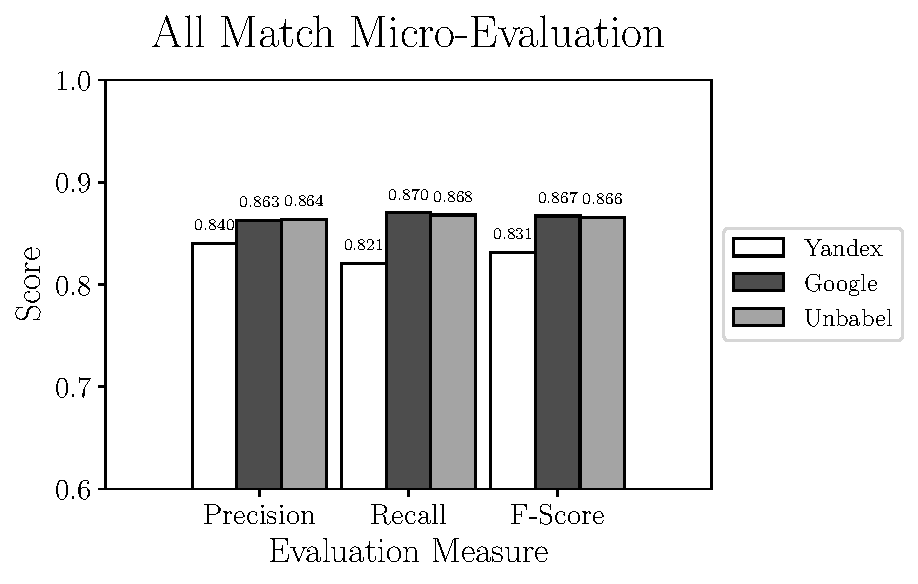
\includegraphics{SupportFiles/plots/all_match_micro_total_plot.pdf}

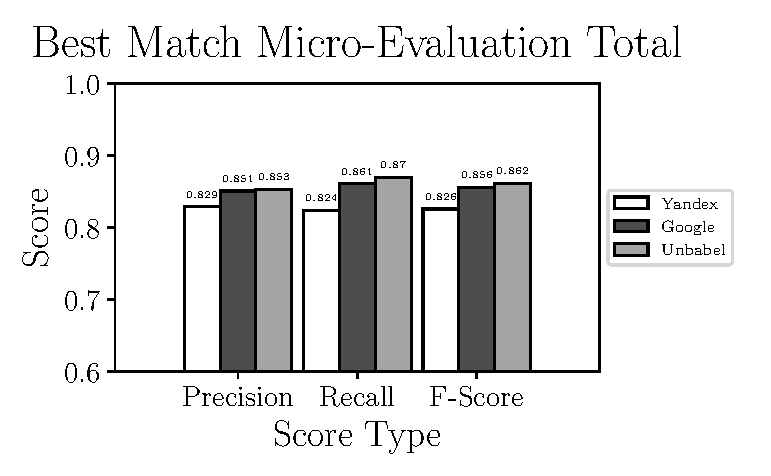
\includegraphics{SupportFiles/plots/best_match_micro_total_plot.pdf}

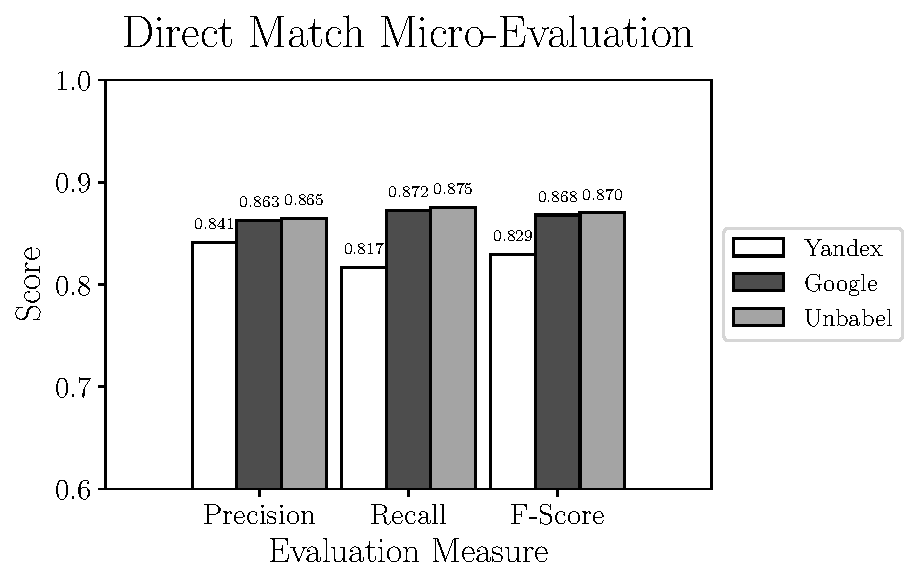
\includegraphics{SupportFiles/plots/direct_match_micro_total_plot.pdf}


The terms extracted from Google translations are more similar to the ones extracted from HT translations than the ones from Yandex translations. This could be just because the human translators used Google Translator to help them in their translation process. This argument loses strength is we assume Google Translate translation outputs changed since the articles were human translated (publication years of the articles used range from 2003 to 2013), but I could not found  data on this. 

The terms extracted from Unbabel and Google translations are really similar, the F-Scores being almost equal. That the translations are similar is not too surprising since the Post-Editing phase at Unbabel is done after MT translation using Google. What could be surprising is that Unbabel doesn't have a higher score. 

In the Introduction to thesis I've proposed the following hypothesis:

\begin{description}
	\item[Hypothesis:] MT+PE is a good trade-off between quality and cost, compared with MT and HT, for translating radiology reports for the purpose of identifying RadLex terms. 
\end{description}

I've written that for this to be true, "MT+PE quality for the task at hand has to be better than MT quality, enough to compensate its higher cost". This does not hold. For this task, if someone had to choose between Google and Unbabel, this someone would be better off using Google since it is cheaper. 

I've also written that for the hypothesis to be true, "MT+PE quality for the task at hand has to be close enough to HT quality". We've already saw that for this specific task, using MT+PE is not worth it. But the question remains, is it worth to use Google MT? The terms extracted from the Google translations are more similar to the ones from HT translation than Yandex, but they are not extremely similar. If this matters probably depends on the practical application the results of this task would have. 

I will now focus on the "Clinical Finding" and "Anatomical Entity" subtrees of RadLex. These are two of the subtrees that probably would be more important when applying RadLex to a Information Retrieval system. 

\subsection{Clinical Finding and Anatomical Entity Subtrees}

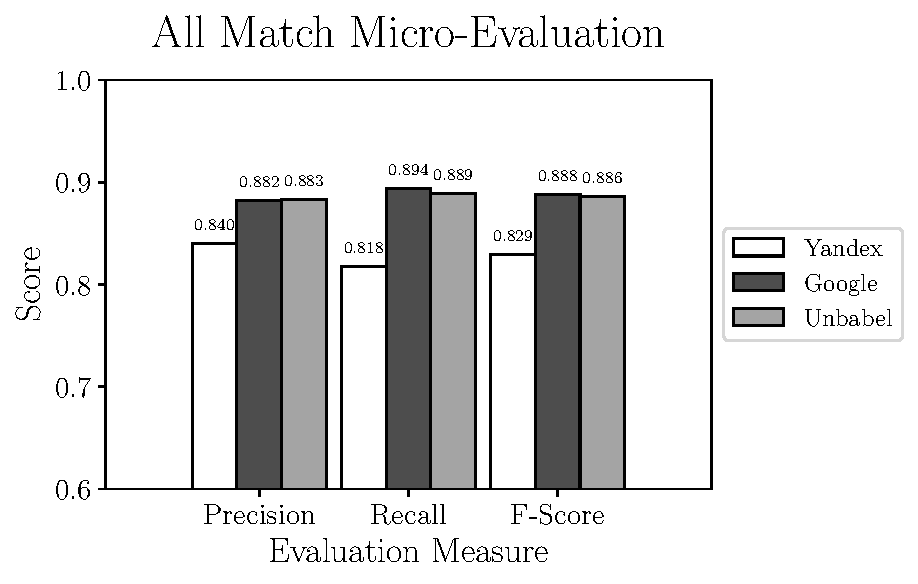
\includegraphics{SupportFiles/plots/all_match_micro_clinical_anatomical_subtrees_plot.pdf}

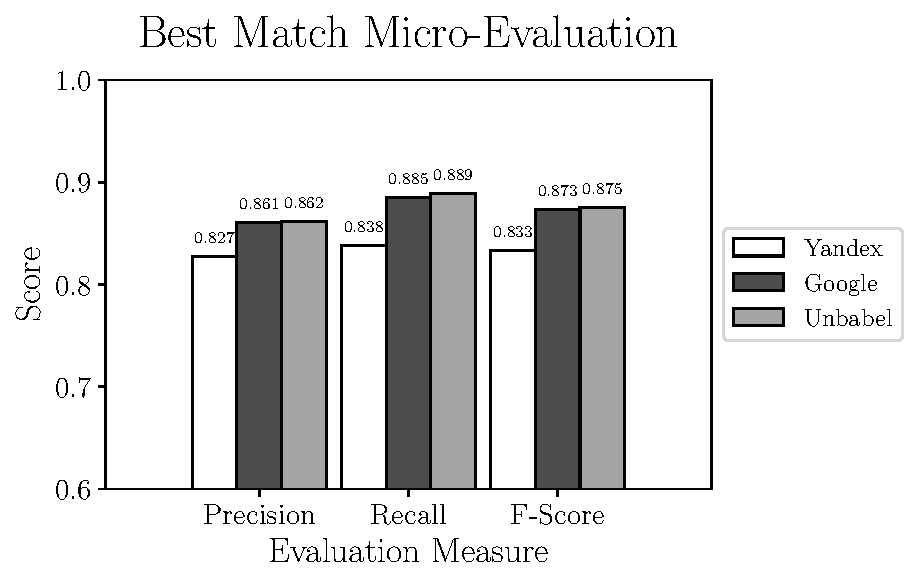
\includegraphics{SupportFiles/plots/best_match_micro_clinical_anatomical_subtrees_plot.pdf}

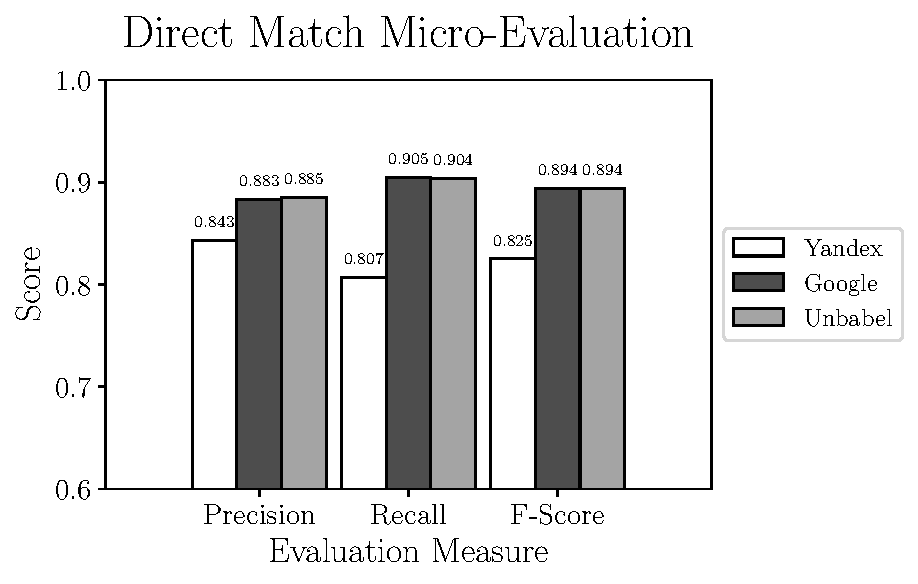
\includegraphics{SupportFiles/plots/direct_match_micro_clinical_anatomical_subtrees_plot.pdf}

Depending on the type of annotation approach and translation it was found between 35.25 and 55.55 "clinical finding" or "anatomical entity" terms per document. The scores obtained are similar to the ones obtained for all terms, with Yandex translation extracted terms being the less similar to the HT translation extracted terms and Google and Unbabel having similar scores. But why these scores? Why do the terms extracted from the MT and MT+PE translated texts are not more similar to the ones extracted from the HT translated texts? 


\section{Discussion}





\section{Conclusions}




  
